\subsubsection{TriState}
\index{TriState@\te{TriState} (package)}

{\bf Package}


\begin{verbatim}
import TriState :: * ;
\end{verbatim}

{\bf Description}

The \te{TriState} package  implements a
tri-state buffer, as shown in Figure \ref{tristate}.  Depending on the
value of the \te{output\_enable},  \te{inout} can be an input or an output.

\begin{figure}[ht]
\begin{center}
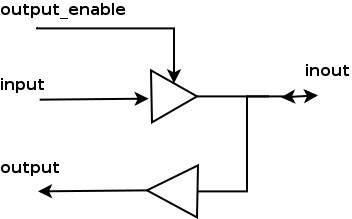
\includegraphics[width = 2 in]{LibFig/tristate}
\caption{TriState Buffer}
\label{tristate}
\end{center}
\end{figure}


The buffer has two
inputs,  an \te{input} of type \te{value\_type} and a Boolean
\te{output\_enable} which  determines the direction
of \te{inout}.  If 
\te{output\_enable} is True, the signal is 
coming in from  \te{input} and out through  \te{inout} and 
 \te{output}.  
 If  \te{output\_enable} is False, then a value can be driven in
 from  \te{inout}, and the \te{output} value will be the value of
  \te{inout}.  The behavior is described  in the tables below.  

\begin{center}
\begin{tabular}{|c|c||c|}
\hline
\multicolumn{3}{|c|}{output\_enable = 0}\\
\multicolumn{3}{|c|}{output = inout}\\
\hline
\multicolumn{2}{|c||}{Inputs}&\\
\cline{1-2}
input&inout&output\\
\hline
0&0&0\\
0&1&1\\
1&0&0\\
1&1&1\\
\hline
\end{tabular}
\end{center}

\begin{center}
\begin{tabular}{|c||c|c|}
\hline
\multicolumn{3}{|c|}{output\_enable = 1}\\
\multicolumn{3}{|c|}{output = in}\\
\multicolumn{3}{|c|}{inout = in}\\
\hline
&\multicolumn{2}{|c|}{Outputs}\\
\cline{2-3}
input&inout&output\\
\hline
0&0&0\\
1&1&1\\
\hline
\end{tabular}
\end{center}


This module is not supported in Bluesim.





{\bf Interfaces and Methods}

The \te{TriState} interface is composed of an \te{Inout} interface and
a \te{\_read} method.  The \te{\_read} method is similar to the
\te{\_read} method of a register in that to read the method you reference
  the  interface in an expression.

\index{TriState@\te{TriState} (interface)}
\begin{center}
\begin{tabular}{|p{.9 in}|p{1.4 in}|p{3.0 in}|}
\hline
\multicolumn{3}{|c|}{TriState Interface}\\
\hline
Name & Type & Description\\
\hline
\hline 
\te{io}  & \te{Inout\#(value\_type)} &\te{Inout} subinterface providing a value of  type \te{value\_type} \\
\hline
\te{\_read}&\te{value\_type}&Returns the value of \te{output} \\
\hline
\end{tabular}
\end{center}

\begin{libverbatim}
(* always_ready, always_enabled *)
interface TriState#(type value_type);
   interface Inout#(value_type)   io;
   method    value_type           _read;
endinterface: TriState
\end{libverbatim}


 

{\bf Modules and Functions}

The \te{TriState} package  provides a module constructor function,
\te{mkTriState}, which  provides the \te{TriState} interface.  The
interface includes an \te{Inout} subinterface and the value of \te{output}. 

\index{mkTriState@\te{mkTriState}}

\begin{center}
\begin{tabular}{|p{1 in}|p{4.5 in}|}
 \hline
&\\
\te{mkTriState}  & Creates a module which provides the
\te{TriState} interface.\\
\cline{2-2}
&\begin{libverbatim}
module mkTriState#(Bool output_enable, value_type input)
                  (TriState#(value_type))
   provisos(Bits#(value_type, size_value));
\end{libverbatim}
\\
\hline
\end{tabular}
\end{center}


{\bf Verilog Modules}

The \te{TriState} module is implemented by the Verilog module
\te{TriState.v} which can be found in the BSC {\V} library, \te{\$BLUESPECDIR/Verilog/}.
